\documentclass{article}

% Packages
\usepackage{graphicx} % For including images
\usepackage{amsmath} % For mathematical symbols and equations

% Title and Author Information
\title{Model Stealing Attack}
\author{Byung Jae Bae}
\date{\today}

\begin{document}

\maketitle

\begin{abstract}
We perform a model stealing attack on a pretrained Resnet50 model by using the KnockoffNet methodology.
\end{abstract}

\section{Introduction}
We run a KnockoffNet attack on a pretrained Resnet50 model trained on the CIFAR dataset with another Resnet50 model but trained on both 
CIFAR and MNIST datasets. We test the new KnockoffNet trained on 10k, 20k, 30k, 40k, and 50k queries to the original pretrained model on the 
CIFAR test dataset, MNIST test dataset, and both combined CIFAR and MNIST test dataset to compare the how the different datasets affect the test accuracies.

\section{Methods}
We used a pretrained Resnet50 model trained on CIFAR dataset from huggingface as our victim model.
We created another Resnet50 model with randomized weights to perform a model stealing attack using 
the KnockoffNet method. The training data was a mix of MNIST and CIFAR data. We recorded the accuracies of 

\section{Results}
The accuracies of the CIFAR test dataset for 10k, 20k, 30k, 40k, and 50k queries were 0.137, 0.1154, 0.151, 0.1797, and 0.161, respectively.
For the MNIST and CIFAR dataset it was 0.1984, 0.18735, 0.18895, 0.23545, and 0.21055.
For only MNIST it was 0.189, 0.1795, 0.1488, 0.2127, 0.2185. The table below makes a clearer illustration.

\begin{figure}
    \begin{center}
        \begin{tabular}{|c | c c c|} 
        \hline
        Number of Queries & CIFAR & MNIST and CIFAR & MNIST \\ [0.5ex] 
        \hline
        10000 & 0.137 & 0.1984 & 0.189 \\ 
        \hline
        20000 & 0.1154 & 0.18735 & 0.1795 \\
        \hline
        30000 & 0.151 & 0.18895 & 0.1488 \\
        \hline
        40000 & 0.1797 & 0.23545 & 0.2127 \\
        \hline
        50000 & 0.161 & 0.21055 & 0.2185 \\ [1ex] 
        \hline
        \end{tabular}
    \end{center}
    \caption{Table of accuracies for different number of queries.}
    \label{fig:table1}
\end{figure}


\begin{figure}
    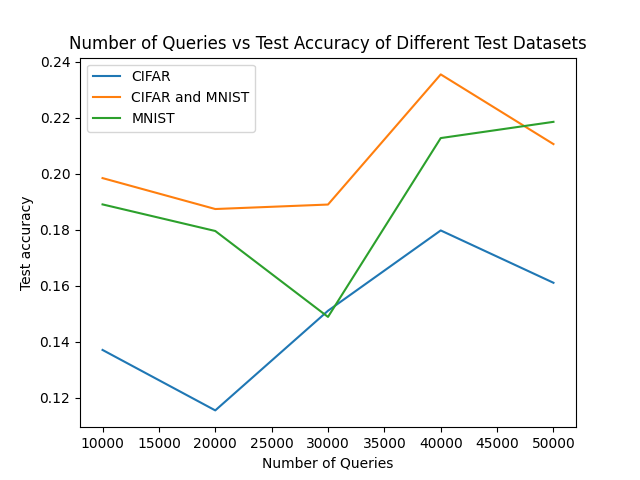
\includegraphics[width=\linewidth]{acc.png}
    \caption{Graph of accuracies for different number of queries.}
    \label{fig:graph1}
\end{figure}

\section{Discussion}
The results were somewhat surprising. Firstly, the accuracies for all test accuracies were very low even for 50k queries.
Secondly, there were no linear trends between number of queries and test accuracies, as the test accuracies would fluctuate throughout
the different query numbers. Despite no linear trends the overall trend seems still to trend positively which would be consistent with our expectations.
One aspect of our training that was imposed was to use MNIST and CIFAR to replicate a model only trained on CIFAR. This most likely have affected our testing accuracies 
because our Knockoff Model was training on out of distribution data compared to what the original model was made for. Since we first feed the MNIST data to the pretrained model 
only trained on CIFAR, the output would likely be incorrect as it was not trained for the task, but downstream our model was fed the incorrect output leading to a worse model to generalize 
to MNIST. This is why MNIST almost consistently scored the lowest accuracy out of the 3 test datasets.


\end{document}